\documentclass[11pt,compress,t,notes=noshow, xcolor=table]{beamer}
\usepackage[]{graphicx}\usepackage[]{color}
%% maxwidth is the original width if it is less than linewidth
%% otherwise use linewidth (to make sure the graphics do not exceed the margin)
\makeatletter
\def\maxwidth{ %
  \ifdim\Gin@nat@width>\linewidth
    \linewidth
  \else
    \Gin@nat@width
  \fi
}
\makeatother

\definecolor{fgcolor}{rgb}{0.345, 0.345, 0.345}
\newcommand{\hlnum}[1]{\textcolor[rgb]{0.686,0.059,0.569}{#1}}%
\newcommand{\hlstr}[1]{\textcolor[rgb]{0.192,0.494,0.8}{#1}}%
\newcommand{\hlcom}[1]{\textcolor[rgb]{0.678,0.584,0.686}{\textit{#1}}}%
\newcommand{\hlopt}[1]{\textcolor[rgb]{0,0,0}{#1}}%
\newcommand{\hlstd}[1]{\textcolor[rgb]{0.345,0.345,0.345}{#1}}%
\newcommand{\hlkwa}[1]{\textcolor[rgb]{0.161,0.373,0.58}{\textbf{#1}}}%
\newcommand{\hlkwb}[1]{\textcolor[rgb]{0.69,0.353,0.396}{#1}}%
\newcommand{\hlkwc}[1]{\textcolor[rgb]{0.333,0.667,0.333}{#1}}%
\newcommand{\hlkwd}[1]{\textcolor[rgb]{0.737,0.353,0.396}{\textbf{#1}}}%
\let\hlipl\hlkwb

\usepackage{framed}
\makeatletter
\newenvironment{kframe}{%
 \def\at@end@of@kframe{}%
 \ifinner\ifhmode%
  \def\at@end@of@kframe{\end{minipage}}%
  \begin{minipage}{\columnwidth}%
 \fi\fi%
 \def\FrameCommand##1{\hskip\@totalleftmargin \hskip-\fboxsep
 \colorbox{shadecolor}{##1}\hskip-\fboxsep
     % There is no \\@totalrightmargin, so:
     \hskip-\linewidth \hskip-\@totalleftmargin \hskip\columnwidth}%
 \MakeFramed {\advance\hsize-\width
   \@totalleftmargin\z@ \linewidth\hsize
   \@setminipage}}%
 {\par\unskip\endMakeFramed%
 \at@end@of@kframe}
\makeatother

\definecolor{shadecolor}{rgb}{.97, .97, .97}
\definecolor{messagecolor}{rgb}{0, 0, 0}
\definecolor{warningcolor}{rgb}{1, 0, 1}
\definecolor{errorcolor}{rgb}{1, 0, 0}
\newenvironment{knitrout}{}{} % an empty environment to be redefined in TeX

\usepackage{alltt}
\newcommand{\SweaveOpts}[1]{}  % do not interfere with LaTeX
\newcommand{\SweaveInput}[1]{} % because they are not real TeX commands
\newcommand{\Sexpr}[1]{}       % will only be parsed by R



\usepackage[english]{babel}
\usepackage[utf8]{inputenc}

\usepackage{dsfont}
\usepackage{verbatim}
\usepackage{amsmath}
\usepackage{amsfonts}
\usepackage{csquotes}
\usepackage{multirow}
\usepackage{longtable}
\usepackage{enumerate}
\usepackage[absolute,overlay]{textpos}
\usepackage{psfrag}
\usepackage{algorithm}
\usepackage{algpseudocode}
\usepackage{eqnarray}
\usepackage{arydshln}
\usepackage{tabularx}
\usepackage{placeins}
\usepackage{tikz}
\usepackage{setspace}
\usepackage{colortbl}
\usepackage{mathtools}
\usepackage{wrapfig}
\usetikzlibrary{shapes,arrows,automata,positioning,calc,chains,trees, shadows}
\tikzset{
  %Define standard arrow tip
  >=stealth',
  %Define style for boxes
  punkt/.style={
    rectangle,
    rounded corners,
    draw=black, very thick,
    text width=6.5em,
    minimum height=2em,
    text centered},
  % Define arrow style
  pil/.style={
    ->,
    thick,
    shorten <=2pt,
    shorten >=2pt,}
}
\usepackage{subfig}
\usepackage{booktabs}
\usepackage{longtable}
\usepackage{array}
\usepackage{multirow}
\usepackage[table]{xcolor}
\usepackage{wrapfig}
\usepackage{float}
\usepackage{colortbl}
\usepackage{pdflscape}
\usepackage{tabu}
\usepackage{threeparttable}
\usepackage{threeparttablex}
\usepackage[normalem]{ulem}
\usepackage{makecell}

% Defnes macros and environments

% basic latex stuff
\newcommand{\pkg}[1]{{\fontseries{b}\selectfont #1}} %fontstyle for R packages
\newcommand{\lz}{\vspace{0.5cm}} %vertical space
\newcommand{\dlz}{\vspace{1cm}} %double vertical space
\newcommand{\mat}[1]{ %short pmatrix command
  \begin{pmatrix}
    #1
  \end{pmatrix}
}
\newcommand{\oneliner}[1] % Oneliner for important statements
{\begin{block}{}\begin{center}\begin{Large}#1\end{Large}\end{center}\end{block}}


% math spaces
\newcommand{\N}{\mathds{N}}                                                 % N, naturals
\newcommand{\Z}{\mathds{Z}}                                                 % Z, integers
\newcommand{\Q}{\mathds{Q}}                                                 % Q, rationals
\newcommand{\R}{\mathds{R}}                                                 % R, reals
\newcommand{\C}{\mathds{C}}                                                 % C, complex
\newcommand{\HS}{\mathcal{H}}                                               % H, hilbertspace
\newcommand{\continuous}{\mathcal{C}}                                       % C, space of continuous functions
\newcommand{\M}{\mathcal{M}} 												% machine numbers
\newcommand{\epsm}{\epsilon_m} 												% maximum error


% basic math stuff
\newcommand{\xt}{\tilde x}													% x tilde
\def\argmax{\mathop{\sf arg\,max}}                                          % argmax
\def\argmin{\mathop{\sf arg\,min}}                                          % argmin
\newcommand{\sign}{\operatorname{sign}}                                     % sign, signum
\newcommand{\I}{\mathbb{I}}                                                 % I, indicator
\newcommand{\order}{\mathcal{O}}                                            % O, order
\newcommand{\fp}[2]{\frac{\partial #1}{\partial #2}}                        % partial derivative
\newcommand{\pd}[2]{\frac{\partial{#1}}{\partial #2}}						% partial derivative

% sums and products
\newcommand{\sumin}{\sum_{i=1}^n}											% summation from i=1 to n
\newcommand{\sumkg}{\sum_{k=1}^g}											% summation from k=1 to g
\newcommand{\prodin}{\prod_{i=1}^n}											% product from i=1 to n
\newcommand{\prodkg}{\prod_{k=1}^g}											% product from k=1 to g

% linear algebra
\newcommand{\one}{\boldsymbol{1}}                                           % 1, unitvector
\newcommand{\id}{\mathrm{I}}                                                % I, identity
\newcommand{\diag}{\operatorname{diag}}                                     % diag, diagonal
\newcommand{\trace}{\operatorname{tr}}                                      % tr, trace
\newcommand{\spn}{\operatorname{span}}                                      % span
\newcommand{\scp}[2]{\left\langle #1, #2 \right\rangle}                     % <.,.>, scalarproduct
\newcommand{\mat}[1]{ 														% short pmatrix command
	\begin{pmatrix}
		#1
	\end{pmatrix}
}
\newcommand{\Amat}{\bm{A}}													% matrix A
\newcommand{\xv}{\bm{x}}													% vector x (bold)
\newcommand{\yv}{\bm{y}}														% vector y (bold)
\newcommand{\Deltab}{\bm{\Delta}}											% error term for vectors
															

% basic probability + stats
\renewcommand{\P}{\mathds{P}}                                               % P, probability
\newcommand{\E}{\mathds{E}}                                                 % E, expectation
\newcommand{\var}{\mathsf{Var}}                                             % Var, variance
\newcommand{\cov}{\mathsf{Cov}}                                             % Cov, covariance
\newcommand{\corr}{\mathsf{Corr}}                                           % Corr, correlation
\newcommand{\normal}{\mathcal{N}}                                           % N of the normal distribution
\newcommand{\iid}{\overset{i.i.d}{\sim}}                                    % dist with i.i.d superscript
\newcommand{\distas}[1]{\overset{#1}{\sim}}                                 % ... is distributed as ... 
% machine learning

%%%%%% ml - data
\newcommand{\Xspace}{\mathcal{X}}                                           % X, input space
\newcommand{\Yspace}{\mathcal{Y}}                                           % Y, output space
\newcommand{\nset}{\{1, \ldots, n\}}                                        % set from 1 to n
\newcommand{\pset}{\{1, \ldots, p\}}                                        % set from 1 to p
\newcommand{\gset}{\{1, \ldots, g\}}                                        % set from 1 to g
\newcommand{\Pxy}{\P_{xy}}                                                  % P_xy
\newcommand{\xy}{(x, y)}                                                    % observation (x, y)
\newcommand{\xvec}{(x_1, \ldots, x_p)^T}                                    % (x1, ..., xp) 
\newcommand{\D}{\mathcal{D}}                                                % D, data 
\newcommand{\Dset}{\{ (x^{(1)}, y^{(1)}), \ldots, (x^{(n)},  y^{(n)})\}}    % {(x1,y1)), ..., (xn,yn)}, data
\newcommand{\xdat}{\{ x^{(1)}, \ldots, x^{(n)}\}}   						 % {x1, ..., xn}, input data
\newcommand{\ydat}{\mathbf{y}}                                              % y (bold), vector of outcomes
\newcommand{\yvec}{(y^{(1)}, \hdots, y^{(n)})^T}                            % (y1, ..., yn), vector of outcomes
\renewcommand{\xi}[1][i]{x^{(#1)}}                                          % x^i, i-th observed value of x
\newcommand{\yi}[1][i]{y^{(#1)}}                                            % y^i, i-th observed value of y 
\newcommand{\xyi}{(\xi, \yi)}                                               % (x^i, y^i), i-th observation
\newcommand{\xivec}{(x^{(i)}_1, \ldots, x^{(i)}_p)^T}                       % (x1^i, ..., xp^i), i-th observation vector
\newcommand{\xj}{x_j}                                                       % x_j, j-th feature
\newcommand{\xjb}{\mathbf{x}_j}                                             % x_j (bold), j-th feature vecor
\newcommand{\xjvec}{(x^{(1)}_j, \ldots, x^{(n)}_j)^T}                       % (x^1_j, ..., x^n_j), j-th feature vector
\newcommand{\Dtrain}{\mathcal{D}_{\text{train}}}                            % D_train, training set
\newcommand{\Dtest}{\mathcal{D}_{\text{test}}}                              % D_test, test set

%%%%%% ml - models general

% continuous prediction function f
\newcommand{\fx}{f(x)}                                                      % f(x), continuous prediction function
\newcommand{\Hspace}{H}														% hypothesis space where f is from
\newcommand{\fh}{\hat{f}}                                                   % f hat, estimated prediction function
\newcommand{\fxh}{\fh(x)}                                                   % fhat(x)
\newcommand{\fxt}{f(x | \theta)}                                            % f(x | theta)
\newcommand{\fxi}{f(\xi)}                                                   % f(x^(i))
\newcommand{\fxih}{\hat{f}(\xi)}                                            % f(x^(i))
\newcommand{\fxit}{f(x^{(i)} | \theta)}                                     % f(x^(i) | theta)
\newcommand{\fhD}{\fh_{\D}}                                                 % fhat_D, estimate of f based on D
\newcommand{\fhDtrain}{\fh_{\Dtrain}}                                       % fhat_Dtrain, estimate of f based on D

% discrete prediction function h
\newcommand{\hx}{h(x)}                                                      % h(x), discrete prediction function
\newcommand{\hh}{\hat{h}}                                                   % h hat
\newcommand{\hxh}{\hat{h}(x)}                                               % hhat(x)
\newcommand{\hxt}{h(x | \theta)}                                            % h(x | theta)
\newcommand{\hxi}{h(\xi)}                                                   % h(x^(i))
\newcommand{\hxit}{h(x^{(i)} | \theta)}                                     % h(x^(i) | theta)

% yhat
\newcommand{\yh}{\hat{y}}                                                   % y hat for prediction of target
\newcommand{\yih}{\hat{y}}                                                  % y hat for prediction of target

% theta
\newcommand{\thetah}{\hat{\theta}}                                          % theta hat

% densities + probabilities
% pdf of x 
\newcommand{\pdf}{p}                                                        % p
\newcommand{\pdfx}{p(x)}                                                    % p(x)
\newcommand{\pixt}{\pi(x | \theta)}                                         % pi(x|theta), pdf of x given theta

% pdf of (x, y)
\newcommand{\pdfxy}{p(x,y)}                                                 % p(x, y)
\newcommand{\pdfxyt}{p(x, y | \theta)}                                      % p(x, y | theta)
\newcommand{\pdfxyit}{p(\xi, \yi | \theta)}                                 % p(x^(i), y^(i) | theta)

% pdf of x given y
\newcommand{\pdfxyk}{p(x | y=k)}                                            % p(x | y = k)
\newcommand{\lpdfxyk}{\log \pdfxyk}                                         % log p(x | y = k)
\newcommand{\pdfxiyk}{p(\xi | y=k)}                                         % p(x^i | y = k)

% prior probabilities
\newcommand{\pik}{\pi_k}                                                    % pi_k, prior
\newcommand{\lpik}{\log \pik}                                               % log pi_k, log of the prior

% posterior probabilities
\newcommand{\post}{\P(y = 1 | x)}                                           % P(y = 1 | x), post. prob for y=1
\newcommand{\pix}{\pi(x)}                                                   % pi(x), P(y = 1 | x)
\newcommand{\postk}{\P(y = k | x)}                                          % P(y = k | y), post. prob for y=k
\newcommand{\pikx}{\pi_k(x)}                                                % pi_k(x), P(y = k | x)
\newcommand{\pikxt}{\pi_k(x | \theta)}                                      % pi_k(x | theta), P(y = k | x, theta)
\newcommand{\pijx}{\pi_j(x)}                                                % pi_j(x), P(y = j | x)
\newcommand{\pdfygxt}{p(y |x, \theta)}                                      % p(y | x, theta)
\newcommand{\pdfyigxit}{p(\yi |\xi, \theta)}                                % p(y^i |x^i, theta)
\newcommand{\lpdfygxt}{\log \pdfygxt }                                      % log p(y | x, theta)
\newcommand{\lpdfyigxit}{\log \pdfyigxit}                                   % log p(y^i |x^i, theta)
\newcommand{\pixh}{\hat \pi(x)}                                             % pi(x) hat, P(y = 1 | x) hat
\newcommand{\pikxh}{\hat \pi_k(x)}                                          % pi_k(x) hat, P(y = k | x) hat

% residual and margin
\newcommand{\eps}{\epsilon}                                                 % residual, stochastic
\newcommand{\epsi}{\epsilon^{(i)}}                                          % epsilon^i, residual, stochastic
\newcommand{\epsh}{\hat{\epsilon}}                                          % residual, estimated
\newcommand{\yf}{y \fx}                                                     % y f(x), margin
\newcommand{\yfi}{\yi \fxi}                                                 % y^i f(x^i), margin
\newcommand{\Sigmah}{\hat \Sigma}											% estimated covariance matrix
\newcommand{\Sigmahj}{\hat \Sigma_j}										% estimated covariance matrix for the j-th class

% ml - loss, risk, likelihood
\newcommand{\Lxy}{L(y, f(x))}                                               % L(y, f(x)), loss function
\newcommand{\Lxyi}{L(\yi, \fxi)}                                            % L(y^i, f(x^i))
\newcommand{\Lxyt}{L(y, \fxt)}                                              % L(y, f(x | theta))
\newcommand{\Lxyit}{L(\yi, \fxit)}                                          % L(y^i, f(x^i | theta)
\newcommand{\risk}{\mathcal{R}}                                             % R, risk
\newcommand{\riskf}{\risk(f)}                                               % R(f), risk
\newcommand{\riske}{\mathcal{R}_{\text{emp}}}                               % R_emp, empirical risk
\newcommand{\riskef}{\riske(f)}                                             % R_emp(f)
\newcommand{\risket}{\mathcal{R}_{\text{emp}}(\theta)}                      % R_emp(theta)
\newcommand{\riskr}{\mathcal{R}_{\text{reg}}}                               % R_reg, regularized risk
\newcommand{\riskrt}{\mathcal{R}_{\text{reg}}(\theta)}                      % R_reg(theta)
\newcommand{\riskrf}{\riskr(f)}                                             % R_reg(f)
\newcommand{\LL}{\mathcal{L}}                                               % L, likelihood
\newcommand{\LLt}{\mathcal{L}(\theta)}                                      % L(theta), likelihood
\renewcommand{\ll}{\ell}                                                    % l, log-likelihood
\newcommand{\llt}{\ell(\theta)}                                             % l(theta), log-likelihood
\newcommand{\LS}{\mathfrak{L}}                                              % ????????????
\newcommand{\TS}{\mathfrak{T}}                                              % ??????????????
\newcommand{\errtrain}{\text{err}_{\text{train}}}                           % training error
\newcommand{\errtest}{\text{err}_{\text{test}}}                             % training error
\newcommand{\errexp}{\overline{\text{err}_{\text{test}}}}                   % training error

% resampling
\newcommand{\GE}[1]{GE(\fh_{#1})}                                           % Generalization error GE
\newcommand{\GEh}[1]{\widehat{GE}_{#1}}                                     % Estimated train error
\newcommand{\GED}{\GE{\D}}                                                  % Generalization error GE
\newcommand{\EGEn}{EGE_n}                                                   % Generalization error GE
\newcommand{\EDn}{\E_{|D| = n}}                                             % Generalization error GE


% ml - irace
\newcommand{\costs}{\mathcal{C}} % costs
\newcommand{\Celite}{\theta^*} % elite configurations
\newcommand{\instances}{\mathcal{I}} % sequence of instances
\newcommand{\budget}{\mathcal{B}} % computational budget
% ml - bagging, random forest

\newcommand{\bl}[1]{b^{[#1]}(x)}											% baselearner with argument for m
\newcommand{\blm}{\bl{m}}												    % baselearner without argument for m
\newcommand{\blmh}{\hat{b}^{[m]}(x)}										% estimated base learner 

% ml - boosting
\newcommand{\fm}{f^{[m]}}                                                   % prediction in iteration m
\newcommand{\fmh}{\hat{f}^{[m]}}                                            % prediction in iteration m
\newcommand{\fmd}{f^{[m-1]}}                                                % prediction m-1
\newcommand{\fmdh}{\hat{f}^{[m-1]}}                                         % prediction m-1
\newcommand{\bmm}{b^{[m]}}                                                  % basemodel m
\newcommand{\bmmh}{\hat{b}^{[m]}}                                           % basemodel m with hat
\newcommand{\betam}{\beta^{[m]}}                                            % weight of basemodel m
\newcommand{\betamh}{\hat{\beta}^{[m]}}                                     % weight of basemodel m with hat
\newcommand{\betai}[1]{\beta^{[#1]}}                                        % weight of basemodel with argument for m
\newcommand{\errm}{\text{err}^{[m]}}                                        % weighted in-sample misclassification rate
\newcommand{\wm}{w^{[m]}}                                                   % weight vector of basemodel m
\newcommand{\wmi}{w^{[m](i)}}                                               % weight of obs i of basemodel m
\newcommand{\thetam}{\theta^{[m]}}                                          % parameters of basemodel m
\newcommand{\thetamh}{\hat{\theta}^{[m]}}                                   % parameters of basemodel m with hat
\newcommand{\rmm}{r^{[m]}}                                                  % pseudo residuals
\newcommand{\rmi}{r^{[m](i)}}                                               % pseudo residuals
\newcommand{\Rtm}{R_{t}^{[m]}}                                              % terminal-region
\newcommand{\Tm}{T^{[m]}}                                                   %
\newcommand{\ctm}{c_t^{[m]}}                                                % mean, terminal-regions
\newcommand{\ctmh}{\hat{c}_t^{[m]}}                                         % mean, terminal-regions with hat
\newcommand{\ctmt}{\tilde{c}_t^{[m]}}                                       % mean, terminal-regions
\newcommand{\fxk}{f_k(x)}                                                   % f_k(x)
\newcommand{\Lp}{L^\prime}
\newcommand{\Ldp}{L^{\prime\prime}}
\newcommand{\Lpleft}{\Lp_{\text{left}}}
% ml - trees, extra trees

\newcommand{\Np}{\mathcal{N}}												% Parent node N
\newcommand{\Nl}{\Np_1}														% Left node N_1
\newcommand{\Nr}{\Np_2}														% Right node N_2

%\newcommand{\pikN}{\hat{\pi}^\Np}

%\usetheme{lmu-lecture}
\usepackage{../style/lmu-lecture}

\let\code=\texttt
\let\proglang=\textsf

\setkeys{Gin}{width=0.9\textwidth}

\title{Introduction to Machine Learning}
\author{Bernd Bischl, Christoph Molnar}
\institute{Department of Statistics -- LMU Munich}
\date{Winter term 2017/18}

\setbeamertemplate{frametitle}{\expandafter\uppercase\expandafter\insertframetitle}



\begin{document}
% Set style/preamble.Rnw as parent.

% Load all R packages and set up knitr

% This file loads R packages, configures knitr options and sets preamble.Rnw as parent file










\lecturechapter{0}{Additional Material}
\lecture{Dataset Descriptions}


\sloppy

\begin{vbframe}{Boston Housing Data Set}




A widely used dataset to benchmark algorithms is the Boston housing dataset.
The data was originally published 1978 by David Harrison and Daniel Rubinfeld in \textbf{\href{https://www.law.berkeley.edu/files/Hedonic.PDF}{Hedonic Housing Prices and the Demand for Clean Air}}.

This paper investigates the methodological problems associated with the use of
housing market data to \textbf{measure the willingness to pay for clean air}.

\begin{center}
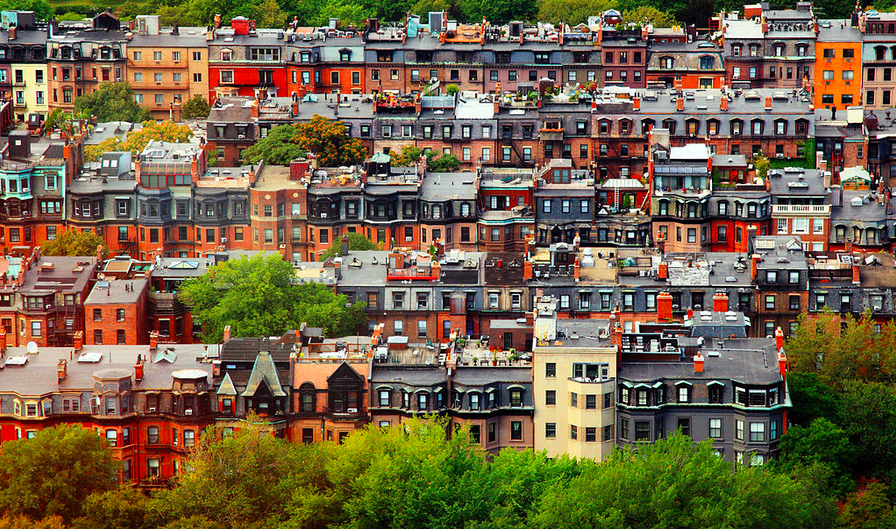
\includegraphics[width=0.425\textwidth]{figure_man/boston_housing.png}
\hspace{0.5cm}
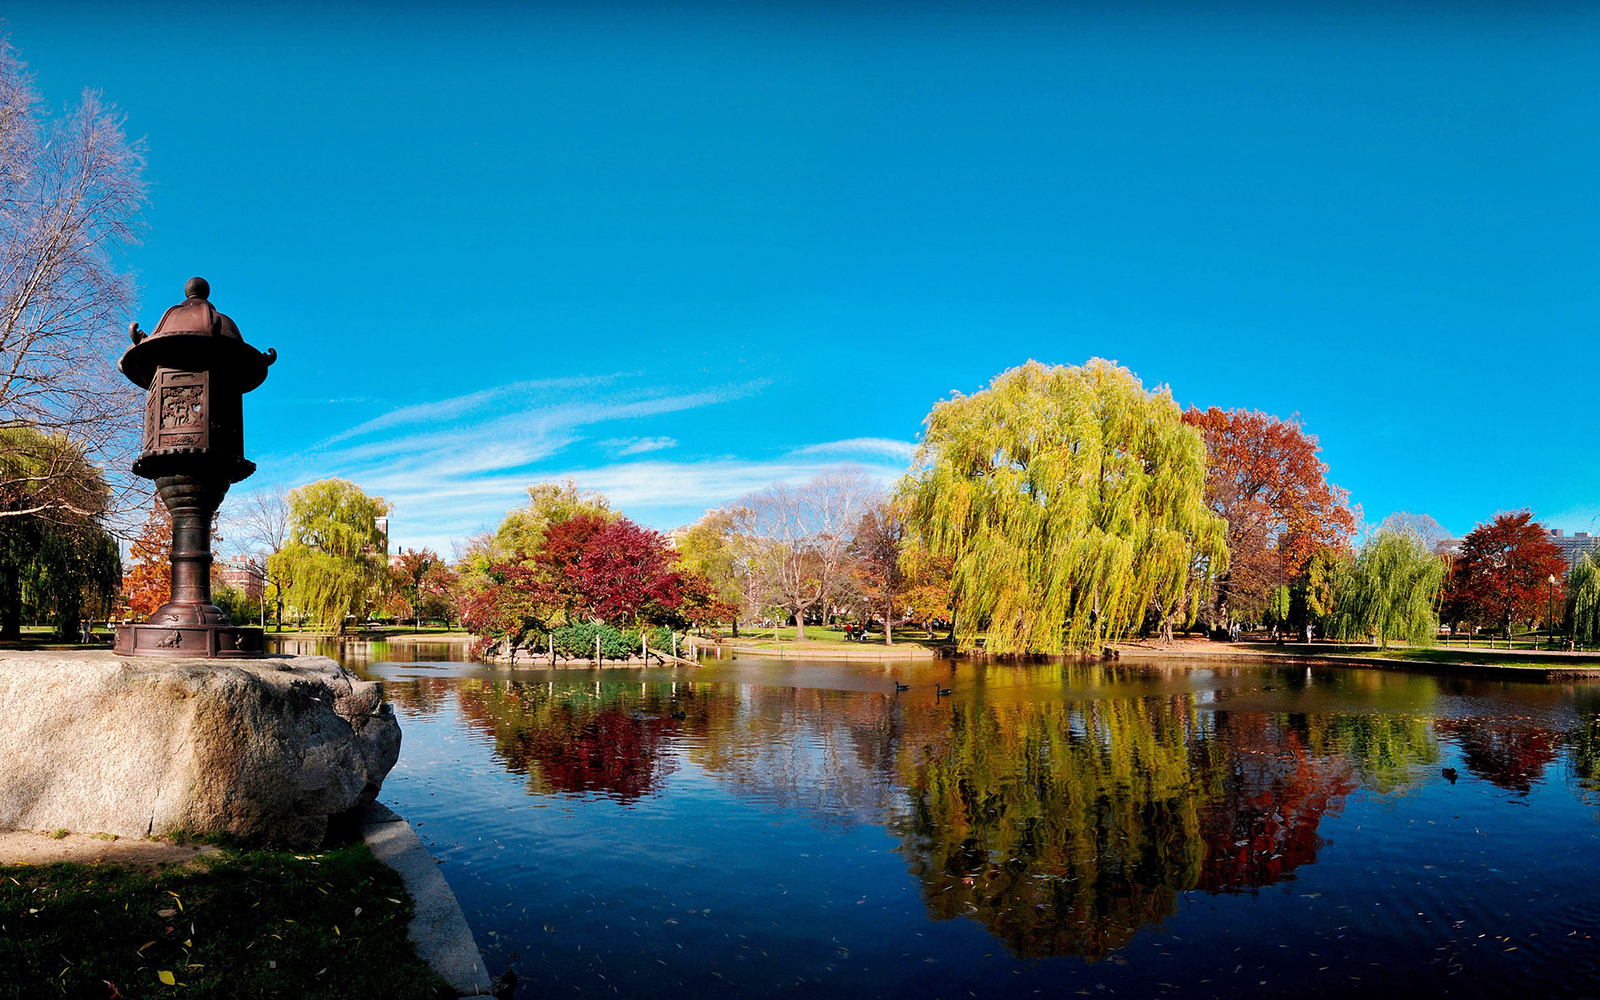
\includegraphics[width=0.402\textwidth]{figure_man/boston_housing_park.jpg}
\end{center}

\framebreak

\textbf{Example Data: Boston Housing}

\begin{table}
  \footnotesize
    \begin{tabularx}{\textwidth}{l:X}
    Variable & Description \\
    \hline
    \textbf{medv} & median value of owner-occupied homes in USD 1000's \\
    crim &	per capita crime rate by town \\
    zn & prop. of residential land zoned for lots over 25,000 sq.ft \\
    indus & proportion of non-retail business acres per town \\
    chas &	Charles River dummy variable (= 1 if tract bounds river; 0 otherwise) \\
    nox & nitric oxides concentration (parts per 10 million) \\
    rm & average number of rooms per dwelling \\
    age & proportion of owner-occupied units built prior to 1940 \\
    dis & weighted distances to five Boston employment centres \\
    rad & index of accessibility to radial highways \\
    tax & full-value property-tax rate per USD 10,000 \\
    ptratio & pupil-teacher ratio by town \\
    b & $1000(B - 0.63)^2$ where B is the prop. of blacks by town \\
    lstat & percentage of lower status of the population \\
    \end{tabularx}
\end{table}

506 obs., 13 features, 'medv' numerical target.

\framebreak

\textbf{Importing the Data}

We use \href{https://www.openml.org}{Open ML} (\href{https://cran.r-project.org/package=OpenML}{R-Package}) to download the dataset in a machine-readable format and convert it into a 'data.frame':


\vfill
\begin{knitrout}\tiny
\definecolor{shadecolor}{rgb}{0.969, 0.969, 0.969}\color{fgcolor}\begin{kframe}
\begin{verbatim}
## # A tibble: 506 x 14
##       CRIM    ZN INDUS CHAS    NOX    RM   AGE   DIS RAD     TAX PTRATIO     B LSTAT  MEDV
##  *   <dbl> <dbl> <dbl> <fct> <dbl> <dbl> <dbl> <dbl> <fct> <dbl>   <dbl> <dbl> <dbl> <dbl>
##  1 0.00632  18    2.31 0     0.538  6.58  65.2  4.09 1       296    15.3  397.  4.98  24  
##  2 0.0273    0    7.07 0     0.469  6.42  78.9  4.97 2       242    17.8  397.  9.14  21.6
##  3 0.0273    0    7.07 0     0.469  7.18  61.1  4.97 2       242    17.8  393.  4.03  34.7
##  4 0.0324    0    2.18 0     0.458  7.00  45.8  6.06 3       222    18.7  395.  2.94  33.4
##  5 0.0690    0    2.18 0     0.458  7.15  54.2  6.06 3       222    18.7  397.  5.33  36.2
##  6 0.0298    0    2.18 0     0.458  6.43  58.7  6.06 3       222    18.7  394.  5.21  28.7
##  7 0.0883   12.5  7.87 0     0.524  6.01  66.6  5.56 5       311    15.2  396. 12.4   22.9
##  8 0.145    12.5  7.87 0     0.524  6.17  96.1  5.95 5       311    15.2  397. 19.2   27.1
##  9 0.211    12.5  7.87 0     0.524  5.63 100    6.08 5       311    15.2  387. 29.9   16.5
## 10 0.170    12.5  7.87 0     0.524  6.00  85.9  6.59 5       311    15.2  387. 17.1   18.9
## # ... with 496 more rows
\end{verbatim}
\end{kframe}
\end{knitrout}
\vfill

\framebreak

\textbf{Exploratory Data Analysis}


Factor variables

\begin{table}[H]
\centering\begingroup\fontsize{7}{9}\selectfont

\begin{tabular}{llll}
\toprule
variable & missing & n\_unique & top\_counts\\
\midrule
CHAS & 0 & 2 & 0: 471, 1: 35, NA: 0\\
RAD & 0 & 9 & 24: 132, 5: 115, 4: 110, 3: 38\\
\bottomrule
\end{tabular}\endgroup{}
\end{table}




Barplots of discrete features

\begin{knitrout}\tiny
\definecolor{shadecolor}{rgb}{0.969, 0.969, 0.969}\color{fgcolor}

{\centering 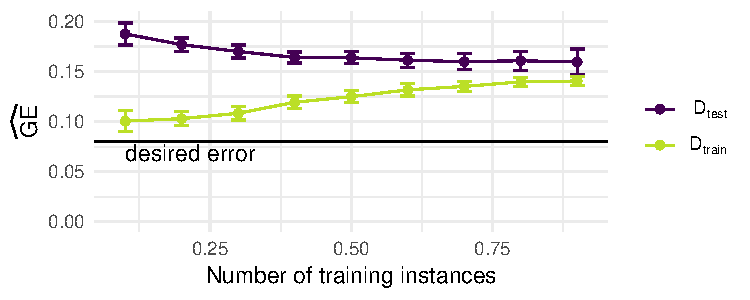
\includegraphics[width=0.95\textwidth]{figure/unnamed-chunk-5-1} 

}



\end{knitrout}

\framebreak

\textbf{Exploratory Data Analysis}


Numeric variables

\begin{table}[H]
\centering\begingroup\fontsize{6}{8}\selectfont

\begin{tabular}{llll}
\toprule
variable & missing & mean & sd\\
\midrule
AGE & 0 & 68.57 & 28.15\\
B & 0 & 356.67 & 91.29\\
CRIM & 0 & 3.61 & 8.6\\
DIS & 0 & 3.8 & 2.11\\
INDUS & 0 & 11.14 & 6.86\\
\addlinespace
LSTAT & 0 & 12.65 & 7.14\\
MEDV & 0 & 22.53 & 9.2\\
NOX & 0 & 0.55 & 0.12\\
PTRATIO & 0 & 18.46 & 2.16\\
RM & 0 & 6.28 & 0.7\\
\addlinespace
TAX & 0 & 408.24 & 168.54\\
ZN & 0 & 11.36 & 23.32\\
\bottomrule
\end{tabular}\endgroup{}
\end{table}



\framebreak

\textbf{Exploratory Data Analysis}


Histograms of numerical features

\begin{knitrout}\tiny
\definecolor{shadecolor}{rgb}{0.969, 0.969, 0.969}\color{fgcolor}

{\centering 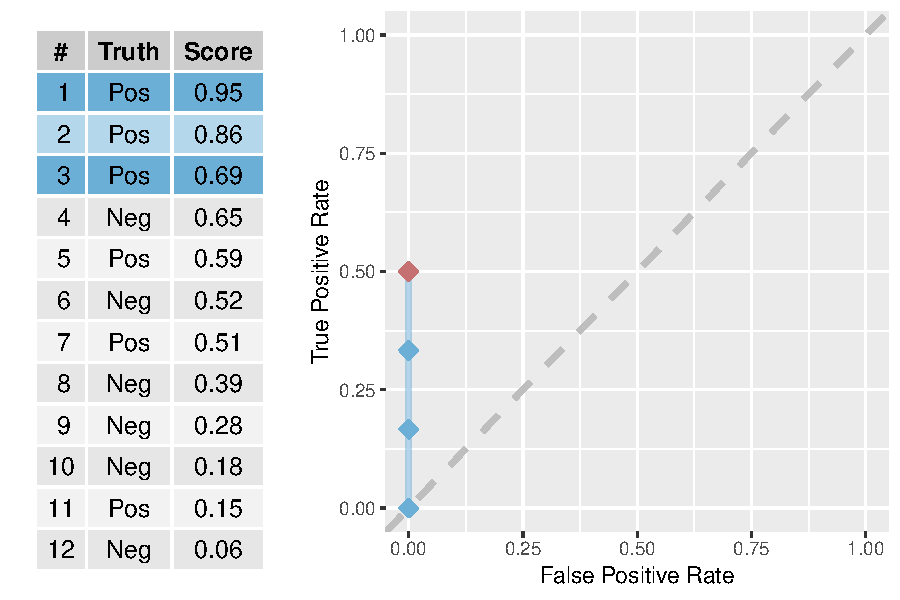
\includegraphics[width=0.95\textwidth]{figure/unnamed-chunk-7-1} 

}



\end{knitrout}


\framebreak

\textbf{Exploratory Data Analysis}


It is always useful to check the correlation among variables:

\begin{knitrout}\tiny
\definecolor{shadecolor}{rgb}{0.969, 0.969, 0.969}\color{fgcolor}

{\centering 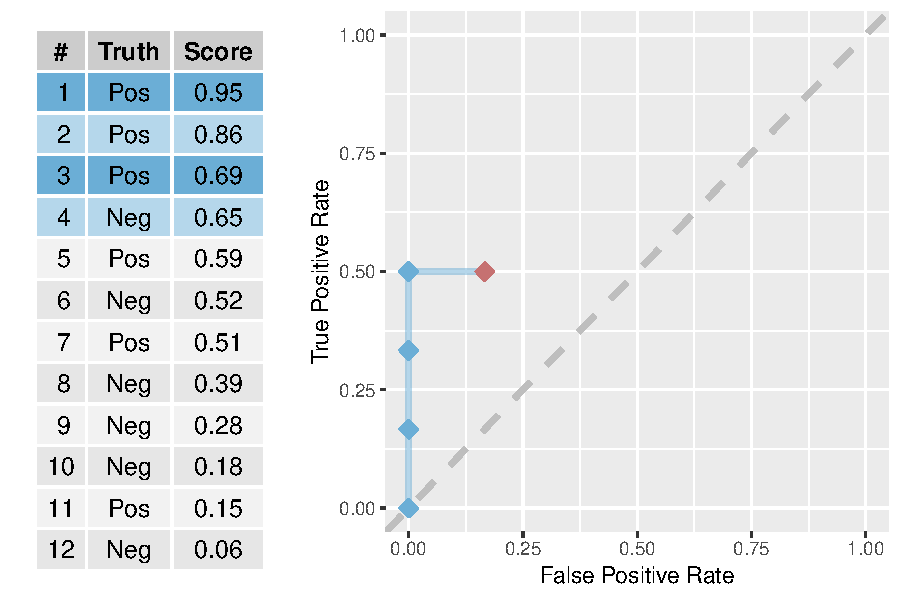
\includegraphics[width=0.95\textwidth]{figure/unnamed-chunk-8-1} 

}



\end{knitrout}

\end{vbframe}

\begin{vbframe}{Iris Data Set}



The iris dataset was introduced by the statistician Ronald Fisher and is one
of the most frequent used datasets. Originally it was designed for linear
discriminant analysis.

The set is a typical test case for many statistical classification techniques
and has its own \textbf{\href{https://en.wikipedia.org/wiki/Iris_flower_data_set}{wikipedia page}}.

\begin{center}
\parbox{0.3\textwidth}{
\centering
  \begin{tabular}{@{}c@{}}
    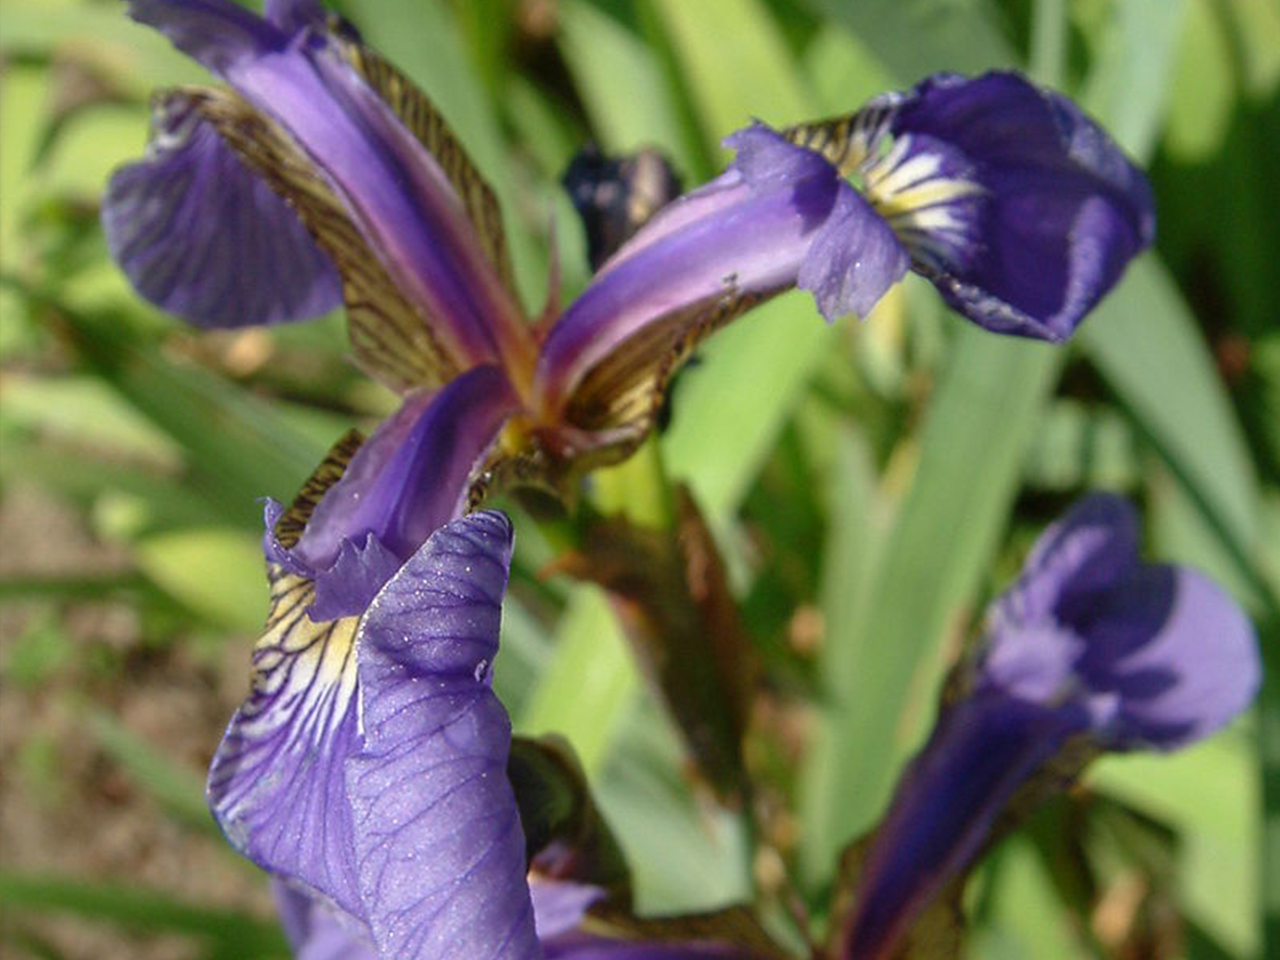
\includegraphics[width=0.25\textwidth]{figure_man/iris_setosa.jpg} \\[\abovecaptionskip]
    \small Setosa
  \end{tabular}
}
\parbox{0.3\textwidth}{
\centering
  \begin{tabular}{@{}c@{}}
    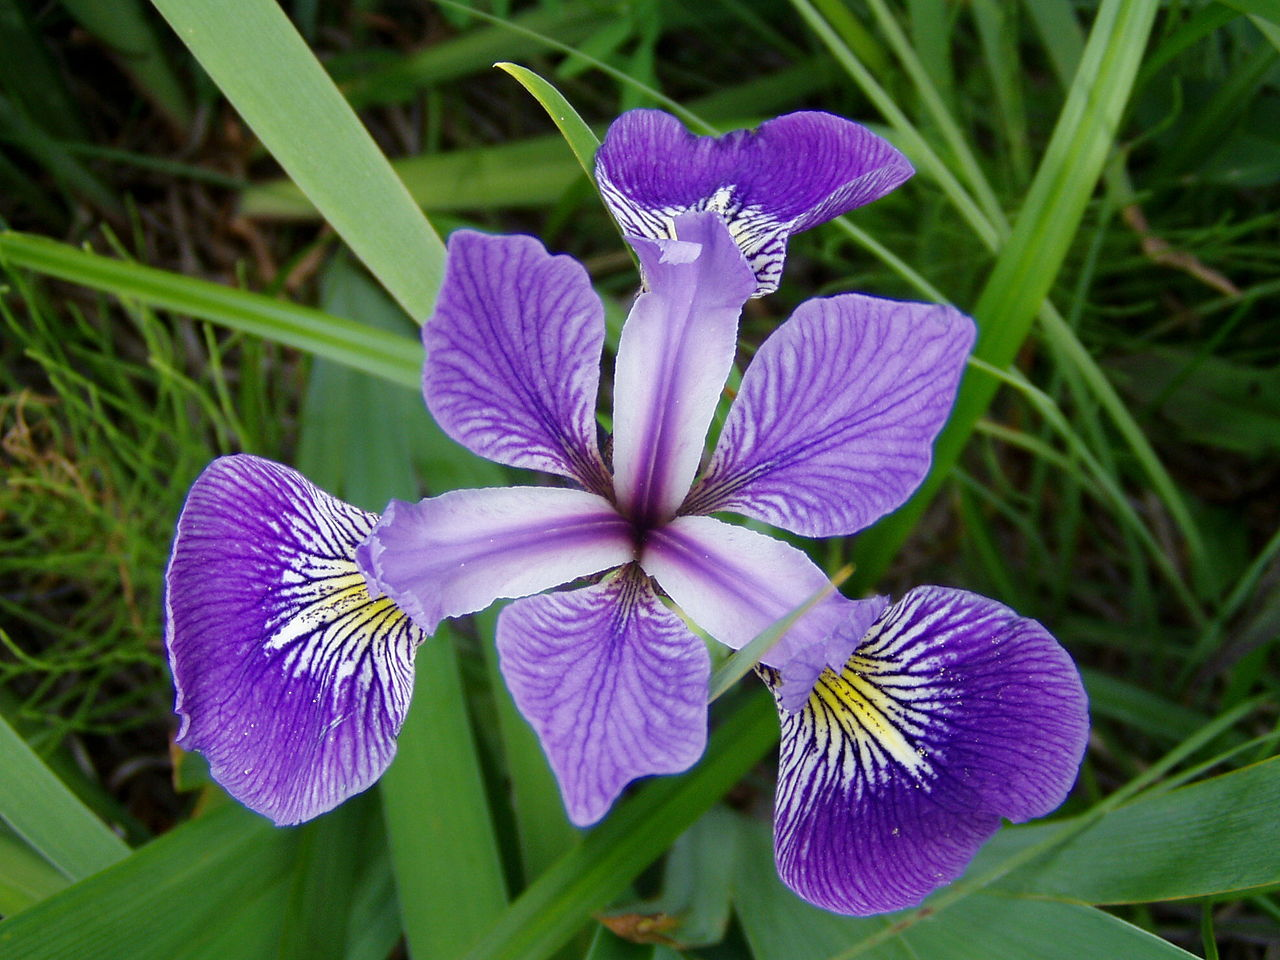
\includegraphics[width=0.25\textwidth]{figure_man/iris_versicolor.jpg} \\[\abovecaptionskip]
    \small Versicolor
  \end{tabular}
}
\parbox{0.3\textwidth}{
\centering
  \begin{tabular}{@{}c@{}}
    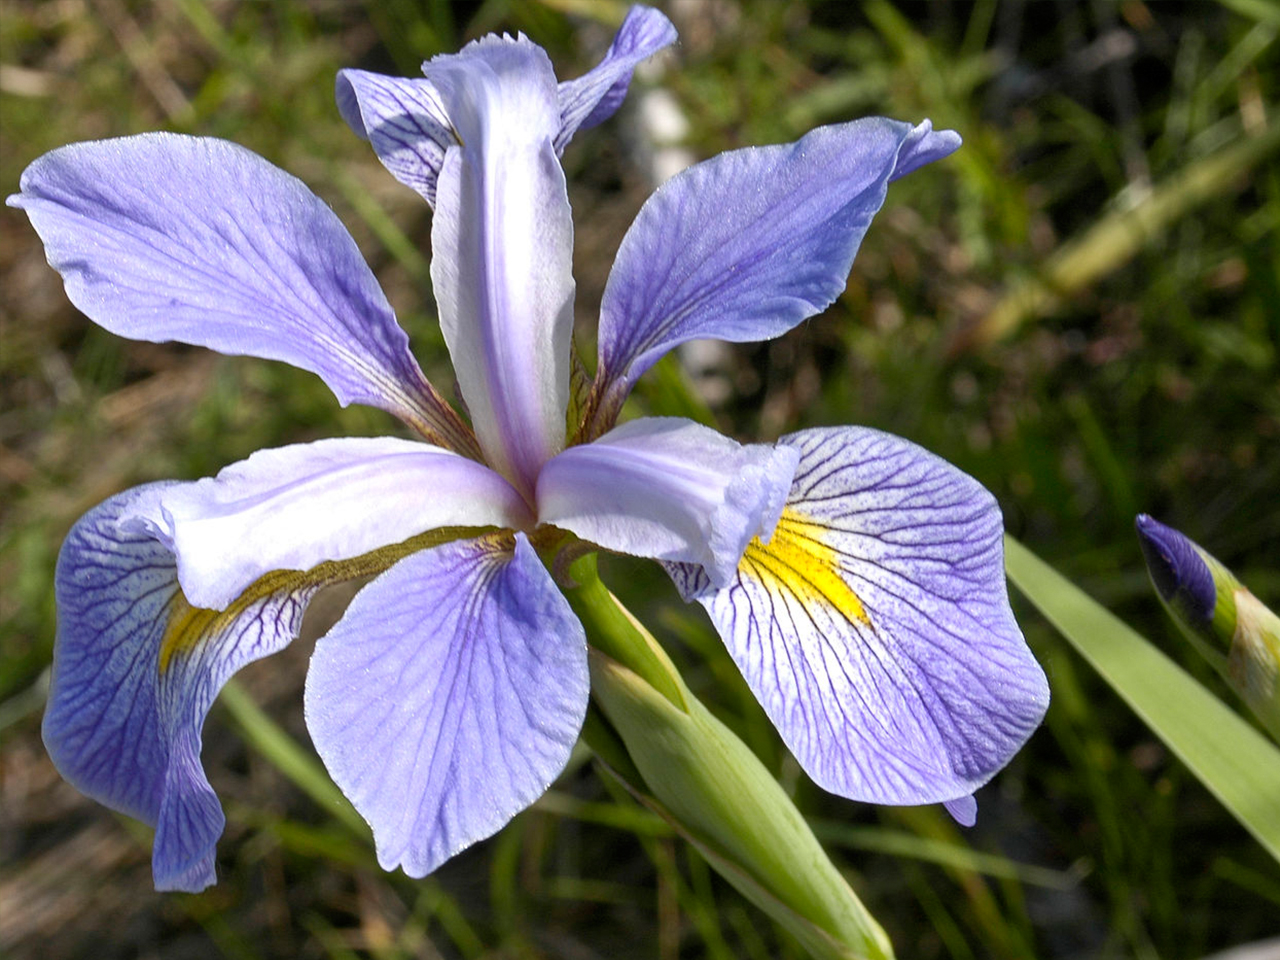
\includegraphics[width=0.25\textwidth]{figure_man/iris_virginica.jpg} \\[\abovecaptionskip]
    \small Virginica
  \end{tabular}
}
\end{center}
Source: \url{https://en.wikipedia.org/wiki/Iris_flower_data_set}

\framebreak

\textbf{Importing the Data}

We use \href{https://www.openml.org}{OpenML} (\href{https://cran.r-project.org/package=OpenML}{R-Package}) to download the dataset in a machine-readable format and convert it into a 'data.frame':


\begin{columns}
  \begin{column}{0.5\textwidth}
    \begin{itemize}
      \item 150 iris flowers (50 setosa, 50 versicolor, 50 virginica),
        species should be predicted.
      \item Sepal length / width and petal length / width in [cm].
    \end{itemize}
  \end{column}
  \begin{column}{0.5\textwidth}
    \begin{center}
      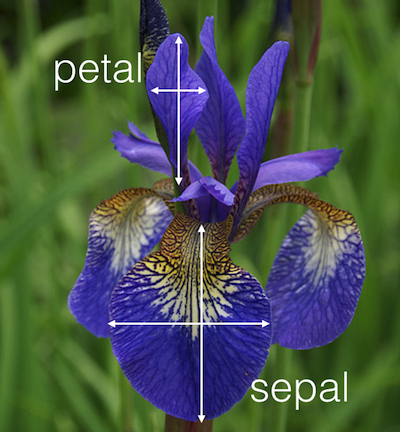
\includegraphics[width=0.6\textwidth]{figure_man/iris_petal_sepal.png}
    \end{center}
  \end{column}
\end{columns}

\vfill

\footnotesize
Source: \url{https://holgerbrandl.github.io/kotlin4ds_kotlin_night_frankfurt//krangl_example_report.html}
\normalsize

\framebreak

\begin{knitrout}\scriptsize
\definecolor{shadecolor}{rgb}{0.969, 0.969, 0.969}\color{fgcolor}\begin{kframe}
\begin{verbatim}
## # A tibble: 150 x 5
##    sepallength sepalwidth petallength petalwidth class      
##  *       <dbl>      <dbl>       <dbl>      <dbl> <fct>      
##  1         5.1        3.5         1.4        0.2 Iris-setosa
##  2         4.9        3           1.4        0.2 Iris-setosa
##  3         4.7        3.2         1.3        0.2 Iris-setosa
##  4         4.6        3.1         1.5        0.2 Iris-setosa
##  5         5          3.6         1.4        0.2 Iris-setosa
##  6         5.4        3.9         1.7        0.4 Iris-setosa
##  7         4.6        3.4         1.4        0.3 Iris-setosa
##  8         5          3.4         1.5        0.2 Iris-setosa
##  9         4.4        2.9         1.4        0.2 Iris-setosa
## 10         4.9        3.1         1.5        0.1 Iris-setosa
## # ... with 140 more rows
\end{verbatim}
\end{kframe}
\end{knitrout}

\framebreak

\textbf{Exploratory Data Analysis}

Factor variables

\begin{table}[H]
\centering\begingroup\fontsize{7}{9}\selectfont

\begin{tabular}{llll}
\toprule
variable & missing & n\_unique & top\_counts\\
\midrule
class & 0 & 3 & Iri: 50, Iri: 50, Iri: 50, NA: 0\\
\bottomrule
\end{tabular}\endgroup{}
\end{table}



\textbf{Exploratory Data Analysis}

Barplots of discrete features

\begin{knitrout}\scriptsize
\definecolor{shadecolor}{rgb}{0.969, 0.969, 0.969}\color{fgcolor}

{\centering 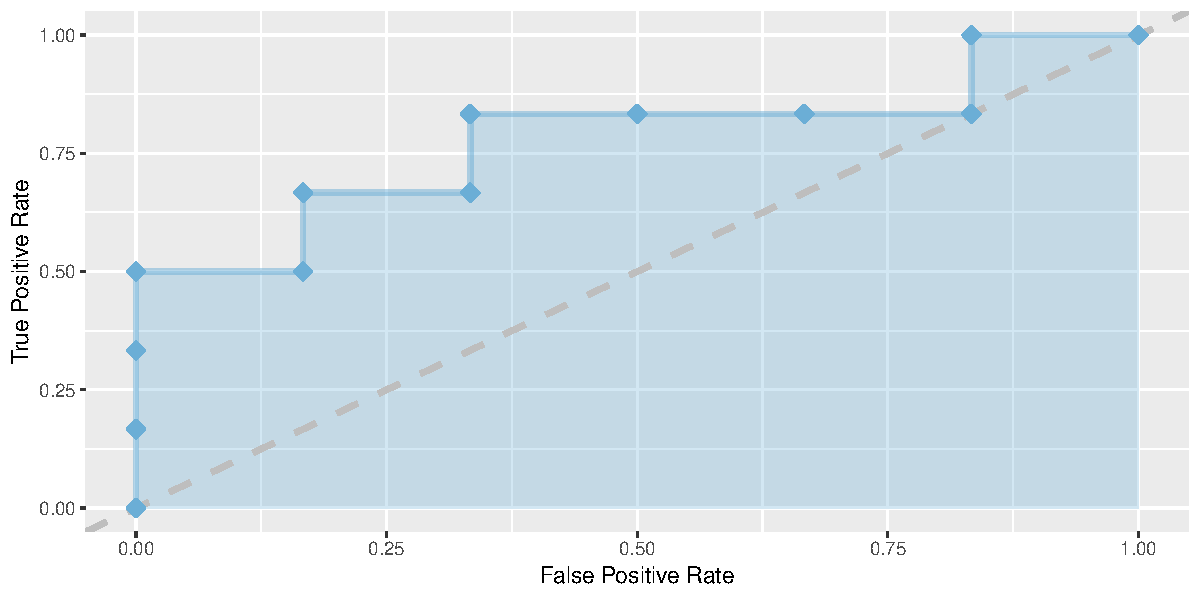
\includegraphics[width=0.95\textwidth]{figure/unnamed-chunk-13-1} 

}



\end{knitrout}

\framebreak

\textbf{Exploratory Data Analysis}

Numeric variables

\begin{table}[H]
\centering\begingroup\fontsize{8}{10}\selectfont

\begin{tabular}{llll}
\toprule
variable & missing & mean & sd\\
\midrule
petallength & 0 & 3.76 & 1.76\\
petalwidth & 0 & 1.2 & 0.76\\
sepallength & 0 & 5.84 & 0.83\\
sepalwidth & 0 & 3.05 & 0.43\\
\bottomrule
\end{tabular}\endgroup{}
\end{table}



\framebreak

\textbf{Exploratory Data Analysis}

Histograms of numerical features

\begin{knitrout}\tiny
\definecolor{shadecolor}{rgb}{0.969, 0.969, 0.969}\color{fgcolor}

{\centering \includegraphics[width=0.95\textwidth]{figure/unnamed-chunk-15-1} 

}



\end{knitrout}



\end{vbframe}

\begin{vbframe}{Spam Data Set}




A data set collected at Hewlett-Packard Labs, that classifies 4601 \textbf{e-mails as spam or non-spam} (variable 'class').
The spam dataset is one of the datasets used in \textbf{The Elements of Statistical Learning} by Trevor Hastie, Robert Tibshirani, and Jerome Friedman.
Besides the option to import it from \textbf{OpenML} it also comes as an example dataset in the packages \textbf{ElemStatLearn} and \textbf{kernlab}.

\framebreak

\begin{itemize}

  \item 'class'      : 0 = no spam, 1 = spam
  \item 'word\_freq\_*': 48 features corresponding to the relative frequency of a specific word in an e-mail
  \item 'char\_freq\_*': 6 features that measures the percentage of a sequence of specific characters occurs relative to the total number of characters
  \item 'capital\_run\_length\_[average, longest, total]': 3 features indicating the average, longest, and sum of uninterrupted sequence of capital letters

\end{itemize}

\framebreak

\textbf{Importing the Data}

We use \href{https://www.openml.org}{Open ML} (\href{https://cran.r-project.org/package=OpenML}{R-Package}) to download the dataset in a machine-readable format and convert it into a 'data.frame':





\begin{itemize}
\item 58 features (e.~g. specific word frequencies)
\item 4,601 observations
\item too much to display as a table

\end{itemize}


\framebreak

\textbf{Exploratory Data Analysis}

Factor variables

\begin{table}[H]
\centering\begingroup\fontsize{7}{9}\selectfont

\begin{tabular}{llll}
\toprule
variable & missing & n\_unique & top\_counts\\
\midrule
class & 0 & 2 & 0: 2788, 1: 1813, NA: 0\\
\bottomrule
\end{tabular}\endgroup{}
\end{table}



\textbf{Exploratory Data Analysis}

Barplots of discrete features

\begin{knitrout}\scriptsize
\definecolor{shadecolor}{rgb}{0.969, 0.969, 0.969}\color{fgcolor}

{\centering \includegraphics[width=0.95\textwidth]{figure/unnamed-chunk-20-1} 

}



\end{knitrout}


\framebreak

\textbf{Exploratory Data Analysis}



The distribution of most variables is highly skewed:

\begin{knitrout}\tiny
\definecolor{shadecolor}{rgb}{0.969, 0.969, 0.969}\color{fgcolor}

{\centering \includegraphics[width=0.95\textwidth]{figure/unnamed-chunk-21-1} 

}



\end{knitrout}


\framebreak

\textbf{Exploratory Data Analysis}



Histograms of numerical features

\begin{knitrout}\tiny
\definecolor{shadecolor}{rgb}{0.969, 0.969, 0.969}\color{fgcolor}

{\centering \includegraphics[width=0.95\textwidth]{figure/unnamed-chunk-22-1} 

}



\end{knitrout}


\framebreak

\textbf{Exploratory Data Analysis}



Histograms of numerical features

\begin{knitrout}\tiny
\definecolor{shadecolor}{rgb}{0.969, 0.969, 0.969}\color{fgcolor}

{\centering \includegraphics[width=0.95\textwidth]{figure/unnamed-chunk-23-1} 

}



\end{knitrout}


\framebreak

\textbf{Exploratory Data Analysis}



Histograms of numerical features

\begin{knitrout}\tiny
\definecolor{shadecolor}{rgb}{0.969, 0.969, 0.969}\color{fgcolor}

{\centering \includegraphics[width=0.95\textwidth]{figure/unnamed-chunk-24-1} 

}



\end{knitrout}


\framebreak

\textbf{Exploratory Data Analysis}



Let's take a look at the correlation among the variables:

\begin{knitrout}\tiny
\definecolor{shadecolor}{rgb}{0.969, 0.969, 0.969}\color{fgcolor}

{\centering \includegraphics[width=0.95\textwidth]{figure/unnamed-chunk-25-1} 

}



\end{knitrout}

\end{vbframe}

\begin{vbframe}{Titanic Data Set}




The original Titanic dataset, describing the \textbf{survival status of individual passengers}(1309) on the Titanic.
The titanic data does not contain information from the crew, but it does contain actual ages of half of the passengers.
The principal source for data about Titanic passengers is the Encyclopedia Titanica.

One of the original sources is Eaton \& Haas (1994) Titanic: Triumph and Tragedy, Patrick Stephens Ltd.
It includes a passenger list created by many researchers (edited by Michael A. Findlay).

\framebreak

\footnotesize
\begin{table}
    \begin{tabularx}{\textwidth}{l:X}
    Variable & Description \\
    \hline
    \textbf{survived}  & 0 = No, 1 = Yes                                                    \\
    pclass    & 1 = 1st; 2 = 2nd; 3 = 3rd                                          \\
    name      & First and last Name                                                \\
    sex       & Sex                                                                \\
    Age       & Age                                                                \\
    sibsp     & Number of Siblings/Spouses Aboard	                                 \\
    parch     & Number of Parents/Children Aboard	                                 \\
    Ticket    & Ticket Number                                                      \\
    fare      & Passenger Fare                                                     \\
    cabin     & Cabin                                                              \\
    embarked  & Port of Embarkation	C = Cherbourg; Q = Queenstown;\newline S = Southampton \\
    body      & Body Identification Number                                         \\
    boat      & Boat number                                                        \\
    home.dest & Home destination                                                   \\
    \end{tabularx}
\end{table}

\framebreak

\textbf{Importing the Data}

We use \href{https://www.openml.org}{Open ML} (\href{https://cran.r-project.org/package=OpenML}{R-Package}) to download the dataset in a machine-readable format and convert it into a 'data.frame':




\begin{knitrout}\tiny
\definecolor{shadecolor}{rgb}{0.969, 0.969, 0.969}\color{fgcolor}\begin{kframe}
\begin{verbatim}
## # A tibble: 1,309 x 14
##    pclass survived name  sex      age sibsp parch ticket  fare cabin embarked boat   body
##  *  <dbl> <fct>    <chr> <fct>  <dbl> <dbl> <dbl> <chr>  <dbl> <chr> <fct>    <chr> <dbl>
##  1      1 1        Alle~ fema~ 29         0     0 24160  211.  B5    S        2        NA
##  2      1 1        Alli~ male   0.917     1     2 113781 152.  C22 ~ S        11       NA
##  3      1 0        Alli~ fema~  2         1     2 113781 152.  C22 ~ S        <NA>     NA
##  4      1 0        Alli~ male  30         1     2 113781 152.  C22 ~ S        <NA>    135
##  5      1 0        Alli~ fema~ 25         1     2 113781 152.  C22 ~ S        <NA>     NA
##  6      1 1        Ande~ male  48         0     0 19952   26.6 E12   S        3        NA
##  7      1 1        Andr~ fema~ 63         1     0 13502   78.0 D7    S        10       NA
##  8      1 0        Andr~ male  39         0     0 112050   0   A36   S        <NA>     NA
##  9      1 1        Appl~ fema~ 53         2     0 11769   51.5 C101  S        D        NA
## 10      1 0        Arta~ male  71         0     0 PC 17~  49.5 <NA>  C        <NA>     22
## # ... with 1,299 more rows, and 1 more variable: home.dest <chr>
\end{verbatim}
\end{kframe}
\end{knitrout}


\framebreak

\textbf{Exploratory Data Analysis}

Factor variables

\begin{table}[H]
\centering\begingroup\fontsize{8}{10}\selectfont

\begin{tabular}{llll}
\toprule
variable & missing & n\_unique & top\_counts\\
\midrule
embarked & 2 & 3 & S: 914, C: 270, Q: 123, NA: 2\\
sex & 0 & 2 & mal: 843, fem: 466, NA: 0\\
survived & 0 & 2 & 0: 809, 1: 500, NA: 0\\
\bottomrule
\end{tabular}\endgroup{}
\end{table}




Barplots of discrete features

\begin{knitrout}\tiny
\definecolor{shadecolor}{rgb}{0.969, 0.969, 0.969}\color{fgcolor}

{\centering \includegraphics[width=0.95\textwidth]{figure/unnamed-chunk-30-1} 

}



\end{knitrout}


\framebreak

\textbf{Exploratory Data Analysis}


Numeric variables

\begin{table}[H]
\centering\begingroup\fontsize{8}{10}\selectfont

\begin{tabular}{llll}
\toprule
variable & missing & mean & sd\\
\midrule
age & 263 & 29.88 & 14.41\\
body & 1188 & 160.81 & 97.7\\
fare & 1 & 33.3 & 51.76\\
parch & 0 & 0.39 & 0.87\\
pclass & 0 & 2.29 & 0.84\\
sibsp & 0 & 0.5 & 1.04\\
\bottomrule
\end{tabular}\endgroup{}
\end{table}




\framebreak

\textbf{Exploratory Data Analysis}


Histograms of numerical features

\begin{knitrout}\tiny
\definecolor{shadecolor}{rgb}{0.969, 0.969, 0.969}\color{fgcolor}

{\centering \includegraphics[width=0.95\textwidth]{figure/unnamed-chunk-32-1} 

}



\end{knitrout}


\framebreak

\textbf{Exploratory Data Analysis}


Seems we have quite some missing observations. Let's take a closer look:

\begin{knitrout}\tiny
\definecolor{shadecolor}{rgb}{0.969, 0.969, 0.969}\color{fgcolor}

{\centering \includegraphics[width=0.95\textwidth]{figure/unnamed-chunk-33-1} 

}



\end{knitrout}


\framebreak

\textbf{Exploratory Data Analysis}


It is always useful to check the correlation among variables:

\begin{knitrout}\tiny
\definecolor{shadecolor}{rgb}{0.969, 0.969, 0.969}\color{fgcolor}

{\centering \includegraphics[width=0.95\textwidth]{figure/unnamed-chunk-34-1} 

}



\end{knitrout}

\end{vbframe}

\endlecture
\end{document}
